\documentclass[12pt, twoside,a4paper]{article}
\oddsidemargin = 10pt
\textwidth = 430pt

\usepackage{fullpage}	 %to make smaller margins
\usepackage{graphicx}
%\usepackage[utf8]{inputenc}
%\usepackage[T1]{fontenc}
%\usepackage{url}

\usepackage[hidelinks]{hyperref}
\usepackage{pdfpages}
\usepackage{placeins}
\usepackage{graphicx}
\usepackage[font=small,labelfont=bf]{caption}
\usepackage{subfig}

%\usepackage{subcaption}
\usepackage{enumerate}
\usepackage{amsmath}
\usepackage{listings} %for showing program code
\usepackage{bm}
\usepackage{wrapfig}
\usepackage{lipsum}
\usepackage{float}
\usepackage{titlesec}	
\usepackage{amsfonts}
\usepackage{amssymb}
\usepackage[comma,authoryear]{natbib}
\usepackage{epstopdf}
\usepackage{array}
\usepackage{blindtext}

%\titlespacing*{\chapter}{0pt}{-10pt}{20pt}
%\titleformat{\chapter}[display]{\normalfont\huge\bfseries}{}{35pt}{}

\setlength{\intextsep}{0pt} %to make wrapfigures beautiful
%\setlength{\oddsidemargin}{0.5cm}
%\setlength{\evensidemargin}{-0.5cm}
\begin{document}
My progress this week. I finished implementing the method. The result had really a lot of artifacts, of which most of them were due to incorrect sampling of textures. Close to the borders, in fact, there are some error due to discretizing everything to a texture that caused the mentioned artifacts. 

The three main artifacts were caused by:
\begin{itemize}
	\item Incorrect sampling of the G-buffer
	\item Incorrect sampling of the cubemap
	\item Shadow bias (when sampling the depth of the texture).
\end{itemize}

I have applied the following fixes:

\section{Incorrect sampling of the G-buffer}

We modify the world coordinate of the point $\mathbf{x}_o$ with normal $\vec{n}_o$ in order to "shrink` a little bit towards the inside of the object according to the light direction $\vec{\omega}_l$:

$$
\mathbf{x}_o' = \mathbf{x}_o - \epsilon_g (\vec{n}_o - \vec{\omega}_l ( \vec{\omega}_l \cdot  \vec{n}_o))
$$

\section{Incorrect sampling of the cubemap}

Since we are sampling a cubemap, we do not need to account for the light direction in this case. In addition, the cubemap needs a 3D vector to be sampled with. So, instead of using $\mathbf{x}_o$, we use a point slightly intruded (i.e. displaced along the normal) in the calculations, according to:

$$
\mathbf{x}_o' = \mathbf{x}_o - \epsilon_c \vec{n}_o
$$

\section{Shadow bias}

In order to avoid artifacts such as shadows acne, we use a bias when comparing the z values of a point to determine if the point is in shadow or not. This implies that we need to convert the depth value from texture space ($\mathbf{z}_{tex}$) to world space again ($\mathbf{z}_{world}$). Since we are using an orthographics camera, the z value is the same in clip coordinates and in normalized device coordinates. Then, we simply use the camera projection properties ($\mathbf{z}_{far}$, $\mathbf{z}_{near}$) to convert the depth into the camera local space, in order to finally add the camera position transformed z value ($\mathbf{z}_{camera}$) and reconstruct the depth in world space:

$$
\mathbf{z}_{world} = \mathbf{z}_{camera} - \frac{\mathbf{z}_{far} - \mathbf{z}_{near}}{2} \left( 2 \mathbf{z}_{tex} - 1 + \frac{\mathbf{z}_{far} + \mathbf{z}_{near}}{\mathbf{z}_{far} - \mathbf{z}_{near}}\right)
$$
		
And finally compare the obtained z with the z position in world space of the point ($\mathbf{z}$) using the bias $\epsilon_b$, so a point is lit iff:

$$
\mathbf{z}_{world} - \epsilon_b < \mathbf{z}
$$		

\begin{figure}
\centering
\subfloat[Without shadow bias and sampling fixes]{
  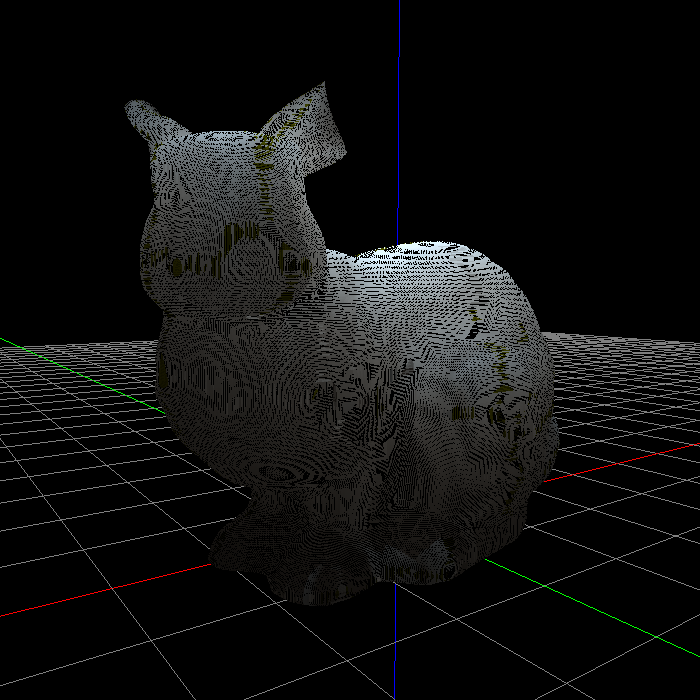
\includegraphics[width=0.45 \linewidth]{all}
  \label{fig:ss2}
} 
\subfloat[With shadow bias and without sampling fixes]{
  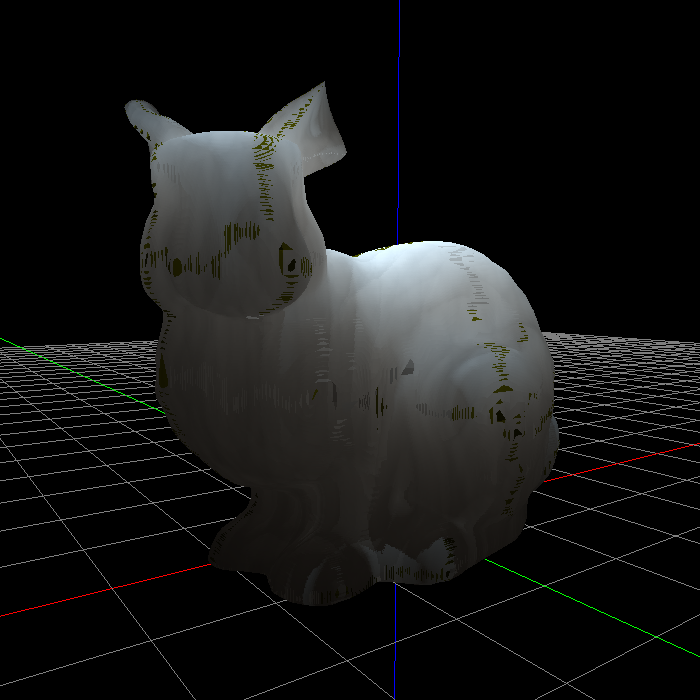
\includegraphics[width=0.45 \linewidth]{nobias}
  \label{fig:ss3}
} 
\\
\subfloat[With both shadow bias and sampling fixes]{
  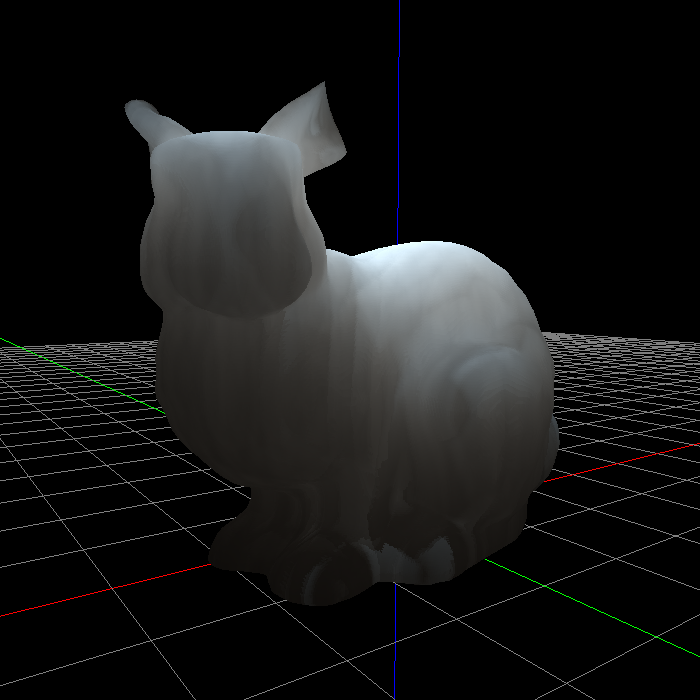
\includegraphics[width=0.45 \linewidth]{cmboffset}
  \label{fig:ss1}
}
\subfloat[Reference]{
  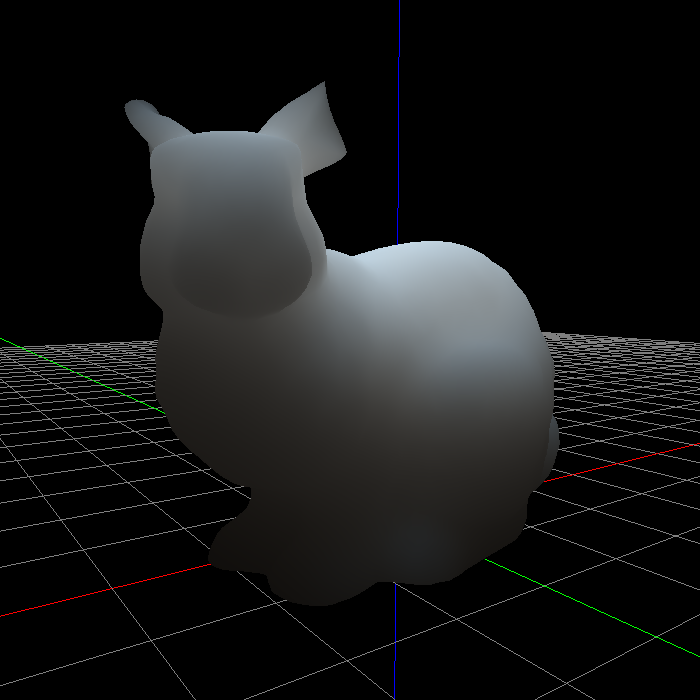
\includegraphics[width=0.45 \linewidth]{reference}
  \label{fig:ss2}
}
\caption{Progressively removing artifacts to get to the final image. }
\label{fig:img}
\end{figure} 

\clearpage
\section{Samples number}

The samples have been arranged to take first the closest to the center of the disc. We can see that with this little thing around 150 samples we stop improving the result, with a radius of 0.5 (in texture space).

\begin{figure}
\centering
\subfloat[10 samples]{
  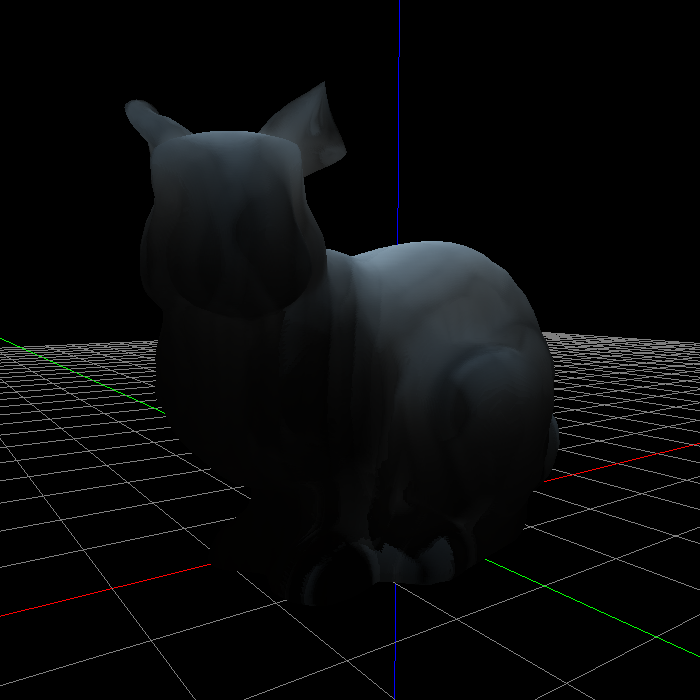
\includegraphics[width=0.25 \linewidth]{10samples}
  \label{fig:ss2}
} 
\subfloat[150 samples]{
  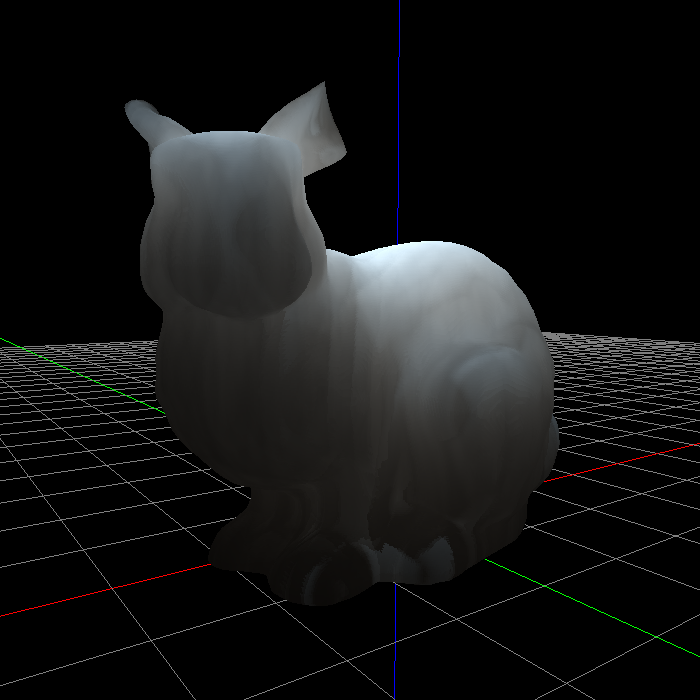
\includegraphics[width=0.25 \linewidth]{150samples}
  \label{fig:ss3}
} 
\subfloat[300 samples]{
  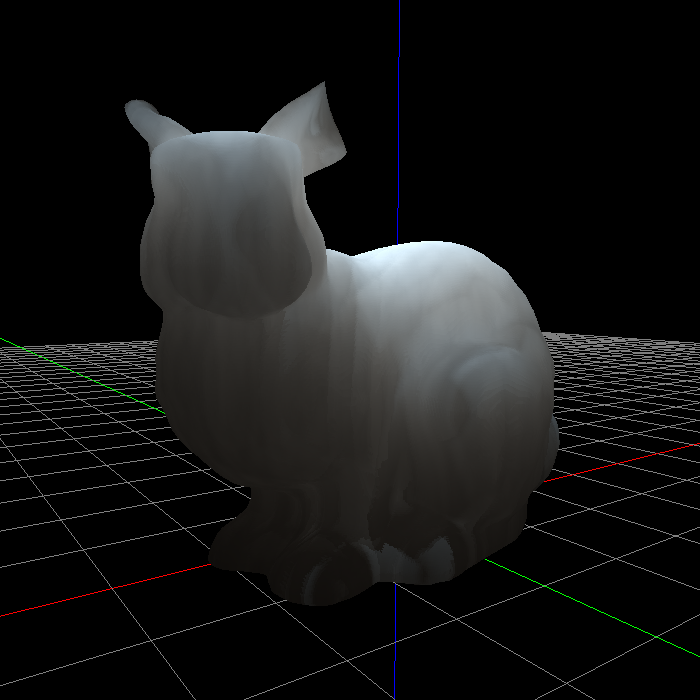
\includegraphics[width=0.25 \linewidth]{300samples}
  \label{fig:ss1}
}
\subfloat[Reference]{
  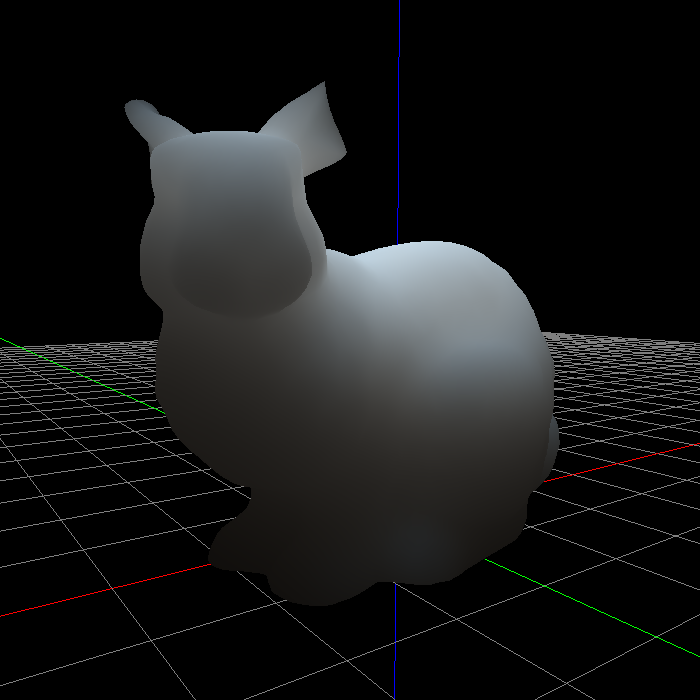
\includegraphics[width=0.25 \linewidth]{reference}
  \label{fig:ss2}
}
\caption{Different results according to the number of samples. }
\label{fig:img}
\end{figure}


\section{Future work}
My schedule for next week:
\begin{itemize}
	\item Solve banding artifacts that are still present (seem to be caused by sampling too close to the point of interest)
	\item Try to add the directional dipole (at the moment I am testing Jensen)
	\item Find reasonable formulas for the epsilons (at the moment they must be set manually)
	\item Focus a little bit more on the report (deliver previous work section and reorganizing some notes on the implementation)
\end{itemize}

\end{document}
